%
% vim:set expandtab tabstop=4 shiftwidth=4:
%


This tutorial provides a brief introduction to the main features of
openBliSSART. We will consider the scenario of speech and music discrimination,
similar to the drum beat separation procedure presented in
\cite{Schuller2009}.


\section{Creating a data set}

In the first step, we will create a data set containing components from speech
and music signals. For this purpose, we will use the ``Browser'' GUI application
which can be found in the {\tt bin} directory of the openBliSSART installation
tree.

Upon starting the browser, you will notice a tree view on the left hand side
which at the first start contains only four entries (nodes), namely
``Classification objects'', ``Labels'', ``Processes'' and ``Responses''. From
this tree view you will be able to access and examine all data that are stored
in the database.

The right hand side of the browser window is used to display and edit the
database objects you have selected in the tree view.


\section{Importing audio files}

To start with, we will now import audio files and separate them into components
using non-negative matrix factorization (NMF).

Simply click the ``Import audio'' button in the lower left corner of the browser
window so that the corresponding ``Import audio'' dialog (figure
\ref{figure:TutorialImportAudio}) appears.

\begin{figure}
    \centering
    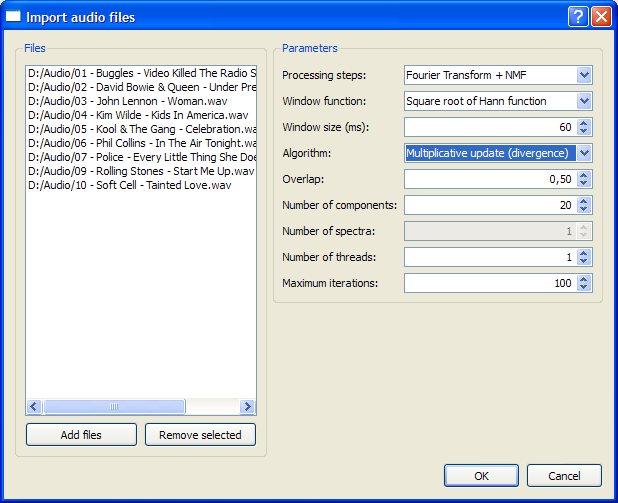
\includegraphics[width=\textwidth]{tutorial-media/ImportAudio.png}
    \caption{%
        \label{figure:TutorialImportAudio}%
        ``Import audio'' dialog
    }
\end{figure}

Ensure that the parameters on the right hand side are set exactly as in figure
\ref{figure:TutorialImportAudio} and select some audio files (WAV or MP3)
containing \emph{music}, preferably around 10-20 seconds long. Then click ``Ok''
and wait for the process to finish. Depending on the number and length of your
audio files, this process may take several minutes as it is computationally
intensive. In order to increase performance on multicore systems, you can adapt
the ``Number of threads'' settings to reflect the number of available cores
before actually starting the process.\\

Once the process has completed, you can expand the ``Classification objects''
node in the tree view so as to examine the entries reflecting the separated
components. The second column states that they are still ``Unlabeled'' --
we will take care of that in the next step.\\

However, at first please repeat the above procedure while this time selecting
audio files containing \emph{speech}. Make sure to remember how many audio files
of each class (speech and music) you have imported as this will simplify the
next step.


\section{Defining classes}

Having imported the neccessary audio files, we will now define the two classes
``Speech'' and ``Music'' by creating two corresponding labels. Click the
``Create label'' button in the lower left corner of the browser window. A new
label entry will be inserted under the ``Labels'' node of the tree view with its
text defaulting to the current date and time. Use the textfield on the right
hand side to change the text to something more meaningful (like ``Music''), then
hit the ``Save'' button. Repeat this step for the ``Speech'' label. The
``Labels'' node should now look like in figure \ref{figure:TutorialLabels}.

\begin{figure}
    \centering
    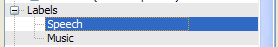
\includegraphics[width=.5\textwidth]{tutorial-media/Labels.png}
    \caption{%
        \label{figure:TutorialLabels}%
        Two defined labels
    }
\end{figure}

Next, we assign these labels to the separated components which we just have
created. Try and select a component in the tree view, and a preview as well as a
list of our labels will then appear on the right hand side (see figure
\ref{figure:TutorialClassificationObjectView}).

\begin{figure}
    \centering
    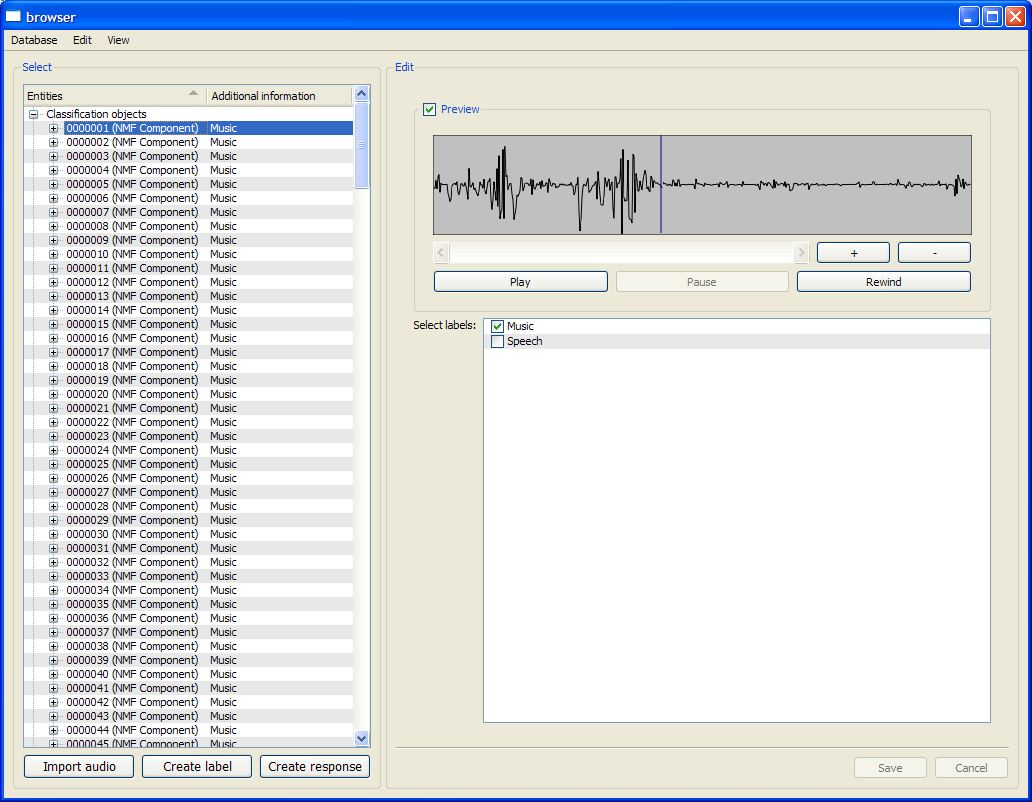
\includegraphics[width=\textwidth]{tutorial-media/ClassificationObjectView.png}
    \caption{%
        \label{figure:TutorialClassificationObjectView}%
        View of a classification object (NMF component)
    }
\end{figure}

Should you want to listen to the selected component, for example to inspect the
results of the NMF procedure, make sure that the ``Preview'' checkbox is
enabled. Once the preview is available, you can listen to the component, move
around, and zoom in and out within the respective signal data by using the
corresponding buttons inside the preview area.\\

While it is possible to assign labels to each component individually using the
checkboxes on the right hand side, for our scenario it is much more convenient
to select all components that were created from music files (remember how many
it were?), then right-click to open the context menu and use the ``Select
label(s)'' item (see figure \ref{figure:TutorialSelectLabels}).

\begin{figure}
    \centering
    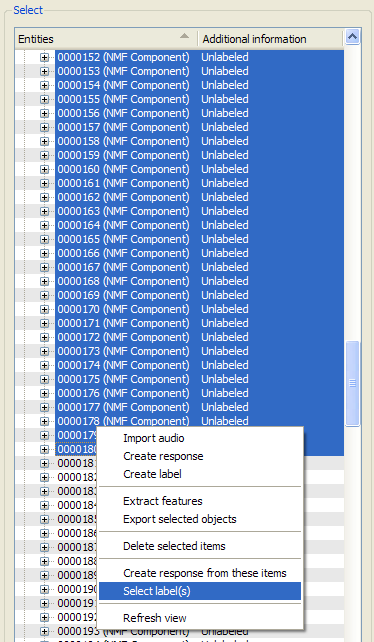
\includegraphics[width=.6\textwidth]{tutorial-media/SelectLabels.png}
    \caption{%
        \label{figure:TutorialSelectLabels}%
        Activating the context menu for components
    }
\end{figure}

A dialog will appear that allows to add one or more labels to all selected
components at the same time. Select ``Music'' and click ``Ok'', then wait for
the operation to finish. Upon completion, all selected components should show
the label ``Music'' instead of ``Unlabeled'' in the second column. By the way,
you can always refresh the tree view by either pressing F5 or selecting
``Refresh view'' from the application's ``View'' menu.\\

Repeat the above procedure for the remaining components, yet this time assign
the label ``Speech''.


\subsection{Feature extraction}

The next step towards creating a data set is to extract features from the
created components. Again, this is very simple: Just select ``Extract features
from all data descriptors'' from the application's ``Database'' menu. Another
dialog will appear, prompting you for the number of feature extraction tasks to
start.  Remember that if you have a multicore system, you might want to set this
number to the number of cores for maximum performance, but usually feature
extraction is done quite fast anyway.\\

After the feature extraction has completed, expand one of the classification
object nodes and in turn also the ``Data descriptors'' node inside. Three
entries will appear: ``Gains'', ``Phase Matrix'' and ``Spectrum''. The phase
matrix is only used for conversion of components to wave files, features are
extracted from either one of the other two elements. Open the nodes ``Gains'' or
``Spectrum''. A list of features with values will be displayed (see figure
\ref{figure:TutorialFeatureSubtree}). The numbers inside the parentheses are
feature parameters (such as the MFCC index). The meanings of the features are
discussed in \cite{Schuller2009}.

\begin{figure}
    \centering
    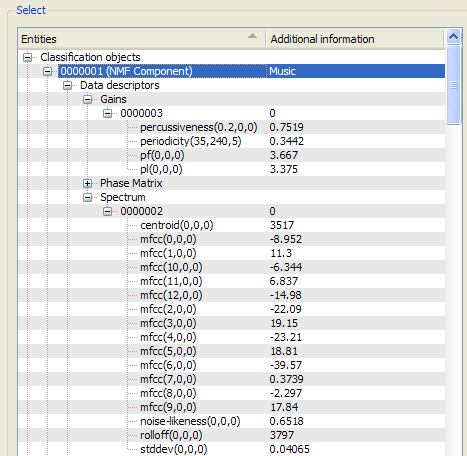
\includegraphics[width=.8\textwidth]{tutorial-media/FeatureSubtree.png}
    \caption{%
        \label{figure:TutorialFeatureSubtree}%
        Feature subtree of a classification object
    }
\end{figure}


\subsection{Defining a response}

Eventually we will have to feed the extracted features to a support vector
machine (SVM). To this end, we create a response variable from all components we
have in the database.

Click the ``Create response'' button in the lower left corner of the browser
window. A response entry will be created under the ``Responses'' node of the
tree view. Like it was the case for labels, the name of the new response
defaults to the current date and time. Use the textfield on the right hand side
to change it into something more meaningful, like for example ``Speech
vs. music'' (see igure \ref{figure:TutorialEditResponse}).

Then click the ``Add CLOs by label'' button and select both labels (``Music''
and ``Speech'') in the corresponding dialog. After clicking ``Ok'', your
response should look like in figure \ref{figure:TutorialEditResponse}.

\begin{figure}
    \centering
    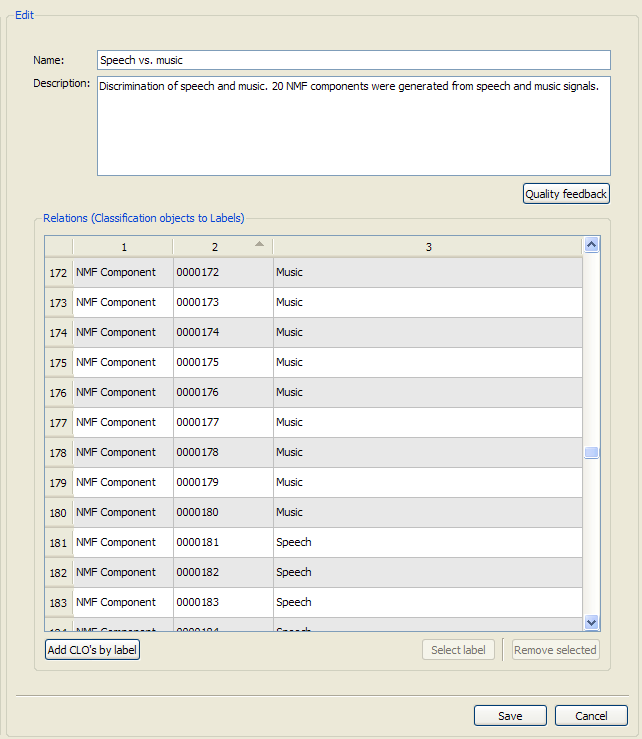
\includegraphics[width=\textwidth]{tutorial-media/EditResponse.png}
    \caption{%
        \label{figure:TutorialEditResponse}%
        Editing a response
    }
\end{figure}


\section{Cross-validation}

To assess the quality of the response we have just defined, we might perform a
stratified 10-fold cross validation. Currently this function is not accessible
from the browser, but is available through a separate tool ({\tt cvtool}).

Open a shell (or Windows command prompt), change to the {\tt bin} directory of
the openBliSSART installation tree and type

\begin{verbatim}
cvtool -r1
\end{verbatim}

assuming the response has the ID\,1, which is the case if it is the first
response you created -- otherwise, check the number appearing before the
respective response's name in the tree view.\\
The cross-validation tool should output something like this:

\verbatiminput{tutorial-media/crossvalidation.txt}


\section{Using a response for blind source separation}

Finally, we are now able to separate audio files into their music and speech
parts by means of the response that we have created.\\

For this purpose, we also use a command-line tool ({\tt septool}). We want the
separation tool to perform NMF into 20 components using a window size of 60\,ms,
then classify the components by a support vector machine trained on the response
we have defined in the previous steps, and eventually create audio files by
summing up all components for each class and transforming them back into the
time domain, i.e. re-synthesizing the results into an appropriate number of
files depending on the number of distinct classes that the given response
uses. Thus the command line for an arbitrary input file \verb|file.wav| is as
follows:

\begin{verbatim}
septool -c20 -s60 -l1 -v file.wav
\end{verbatim}

Again, it is assumed that our response has ID\,1. The {\tt -v} (``volatile'')
option has been added here because we do not want to store additional components
from the given input file \verb|file.wav| into the database.\\

The result of this procedure will be two wave files, namely {\tt
  file\_Speech.wav} and {\tt file\_Music.wav}. Of course, you can replace {\tt
  file.wav} by any suitable WAV or MP3 file. Try mixing speech and music
together and then separating them using the separation tool like described above.\\

\noindent \textbf{Congratulations, you have just finished openBliSSART's
  introductory tutorial. For an in-depth discussion of openBliSSART's features
  and toolbox, move on to the next sections.}
